\chapter{Software}
\label{software}
This part explains the software used in the prototype. It will follow the requirements explained in \autoref{Krav_til_funktionalitet}. The software is based on Arduino (https://www.arduino.cc) and Processing (https://processing.org). The communication between Arduino and Processing happens via a USB A/B connection and the Firmata protocol (http://firmata.org/wiki/Download). The Arduino reads the analogue voltages from the sensors and are via the inbuilt AD converter sent to Processing which process the information. The PC's hardware is used to store, compute and play the audio files by using Processing. This was done in order to make a working prototype faster. 

%Følgende afsnit handler om softwarens opbygning. Afsnittet tager udgangspunkt i de specifikke funktionalitetskrav som står beskrevet i \autoref{Krav_til_funktionalitet}. På baggrund af kravenenes prioritering beskriver først hvordan et system overordnet kan se ud. Dernæst følger en  forklaring af hvordan programkoden virker.
 
%\section{Overordnet system}
%Funktionen, Afspil lyd, prioriteres som den vigtigste funktion hvorfor den implementeres først. Funktionen aktiveres som resultat af at brugeren interagere med en sensor.   
%Programmet baseres på Arduino (https://www.arduino.cc) og Processing (https://processing.org). Kommunikation mellem Arduino og Processing foregår med USB kabel via protokollen Firmata (http://firmata.org/wiki/Download). 
% Arduinoen bruges til at aflæse sensornes analoge spændinger. De målte værdier sendes, via Firmata, videre til Processing som derefter bearbejder informationen.
% Ved at benytte Processing kan PC'ens egen hardware bruges til at bearbejde, lagre og afspille lydfilerne. Denne opsætning er valgt for hurtigt og let at konstruerer en fungerende prototype.  

\section{Walkthrough of the code}
The code has been developed as an iterative process and the following will describe how the software works in small steps. There is a flow chart at the end of the chapter which will be useful when reading this section, see for the flow in the \texttt{draw()} function \autoref{fig:protoFlowChart03.pdf}. The entire code along with a graphical version is attached in the hand-in ZiP-file.
%Programkoden udvikles i en iterativ proces. Følgende giver en forklaring af programkodens indhold og funktion.  
Firstly the Firmata protocol is initialised using StandardFirmata. This allows Processing to access the functionalities of the Arduino. Processing needs to be set up correctly to receive the information. This is done like this:
%Til Arduinoen overføres protokollen Firmata som StandardFirmata. Derved kan funktionaliteten på arduinoen tilgås ved hjælp af Processing. For at  kontakt mellem Arduino og Processing er etableret, er det nødvendigt også at opsætte Processing til kommunikationen. Dette gøres ved at følgende eksekveres:

\begin{figure}[H]
\includegraphics[scale=0.8]{Figure/programkode01.png}
\end{figure}
  
  The libraries \texttt{cc.arduino} and \texttt{processing.serial} are imported and the object \texttt{Arduino} is declared as \texttt{arduino}. Next the object is initialised in the function \texttt{setup()}. The correct port is then chosen from \texttt{Arduino.list()}.
%Først importeres bibliotekerne: cc.arduino og processing.serial.
%Derefter erklæres objektet Arduino som arduino. 
%Til sidst initialiseres objektet i funktionen setup(). Her vælges fra Arduino.list() hvilket port arduinoen er tilsluttet. 
Next step is to be able to play sound files via Processing. This is solved like this:
%Næste skridt er at kunne afspille lydfiler i processing. Det gøres ved at følgende eksekveres:

\begin{figure}[H]
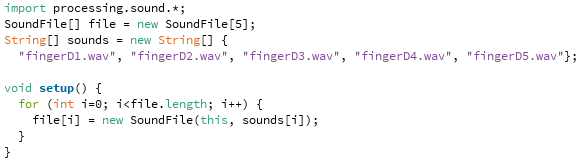
\includegraphics[scale=0.8]{Figure/programkode02.png}
\end{figure}  
 
 The library \texttt{processing.sound} is imported which is needed to play the files. An array of the object \texttt{Soundfile} is declared with the name \texttt{file} with the lenght of five. Next is the name of the files to be played. They need to be in the same folder as the program. They are declared in an array of the \texttt{String} class. Every slot in the array is then matched with the files in the for loop. This loop continues until there are no more space in the \texttt{file} array.
%Først importeres biblioteken: processing.sound.
%Derefter erklæres et array af objektet Soundfile som file, med fem pladser.
%Herefter erklæres et array af klassen Strings som efterfølgende initialiseres med navnene på de lydfiler der skal afspilles i programmet.
%Til sidst initialiseres arrayet file, så hver plads i arrayet pares med en lydfil. Dette sker i funktionen setup via et for loop. Loopet fortsætter så længe der er pladser i arrayet file. 
Now the program is able to communicate with the Arduino and the particular sound files are ready to be played. Further three variables are needed to save  vital information.
% 

\begin{figure}[H]
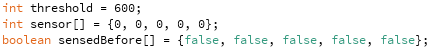
\includegraphics[scale=0.8]{Figure/programkode03.png}
\end{figure}  

The  \texttt{threshold} integer saves the limit set for when a read sensor value is big enough to be played. The integer array \texttt{sensor} is set to zeroes and is used to save the sensor values as the loop progresses. An important feature is the boolean array \texttt{sensedBefore}. This is initially set to \texttt{false} and is used to check if a sensor already have surpassed the threshold value and  played the wanted sound. This is done so that the sound will not keep repeating 60 times a second but only play once when the sensor value is higher than the threshold.
%En integer, threshold, gemmer grænseværdien for hvornår en aflæst sensorværdi er høj nok til at en lyd skal afspilles. 
%Et integer array, sensor, sættes som udgangspunkt til nul og bruges efterfølgende til at gemme hver sensors aflæste værdi. 
%Et boolean array, sensedBefore, sættes som udgangspunkt til false og bruges efterfølgende til at tjekke om en sensorværdi ellerede har overskredet grænseværdien og afspillet en lyd. 
 
%Følgende beskriver forløbet som foregår ved funktionskaldet draw(). Umiddelbart er formålet med koden at afspille en lydfil hvis en aflæst sensorværdi overskrider threshold. Derudover sørger koden for at lydfilen kun afspilles en enkelt gang så længe sensorværdien er over threshold. 

  
The \texttt{draw()} function is a built in function in Processing which is run 60 times a second. A for loop is initialised every time \texttt{draw()} is called. The for loop is made to run once for every place available in the \texttt{sensor} array which starts at zero the first time the loop is run. \texttt{i} then grows one value for every run through. That way \texttt{i} is used as a guide to how many times the loop is run.
%Funktionen draw() er en indbygget funktion i processing som køres 60 gange i sekundet. 
%Hver gang funktionen kaldes, igangsættes et for loop. For loopet er dimensioneret til at køres igennem en enkelt gang for hver plads i arrayet sensor. i, som starter på nul ved første gennemgang af for loopet, har en tilvækst på én ved hver gennemgang. i brugeres efterfølgende som en guide til hvor mange gange for loopet er kørt igennem. 

\begin{figure}[H]
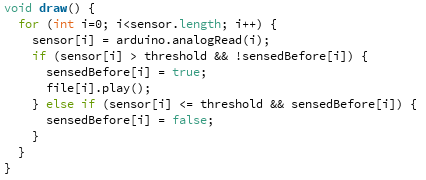
\includegraphics[scale=0.8]{Figure/programkode04.png}
\end{figure}

Firstly the analogue pin is read and the value is stored in the \texttt{sensor} array. The analogue channel is chosen according to \texttt{i} which starts at zero. In the first run through of the loop, this corresponds to the pin A0 (\texttt{analogRead(0)}) and the value is stored in the first spot in the \texttt{sensor} array. Next is the stored value compared to the threshold in an if statement. If  the stored analogue value is bigger than the threshold and the booloean \texttt{sensedBefore[0]} is false, then the code inside the statement is executed. If this is the case then \texttt{sensedBefore[0]} is set to true and the sound file (\texttt{file[0]}) is played. If, however, this is not the case because the sensor value is not bigger than the threshold or because \texttt{sensedBefore} is not false, then again the sensor value is compared to the threshold in an \texttt{else if} statement. This time to check if the value is equal to or lower than the threshold. If it is lower than the threshold and \texttt{sensedBefore[0]} is true, the code in the \texttt{else if} statement is executed. Then \texttt{sensedBefore[0]} is set to false once again.
%Det første der sker i for loopet er at en analog kanal på arduinoen aflæses, og værdien gennes i arrayet sensor. Den analoge kanal vælges ud fra i som til at starte med er 0. Derved aflæses kanal A0, analogRead(0), og gemmes på første plads i arrayet sensor, sensor[0], ved første gennemgang af for loopet. 
%Det næste der sker er at den aflæste sensorværdi sammenlignes med threshold i et if statement. Hvis den aflæste sensorværdi er højere end threshold og booleanen, sensedBefore[0], er false, eksikveres koden inden i if statmentet. Er det tilfældet sættes sensedBefore[0] til true og lydfilen, file[0], afspilles.
%Er det ikke tilfældet, fordi den aflæste sensorværdi ikke er over threshold eller fordi sensedBefore ikke er false, sammenlignes den aflæste sensorværdi igen med threshold i et else if statement. Denne gang for at tjekke om værdien er lig eller lavere end threshold. Hvis den aflæste sensorværdi er lavere end threshold og booleanen, sensedBefore[0], er true, eksikveres koden inden i else if statementet. Er det tilfældet sættes sensedBefore[0] til false.


The loop continues this process for every place in the \texttt{sensor} array. Therfore the second time the loop is run it is \texttt{sensor[1]} which is equal to the value read by pin A1 which is \texttt{analogRead(1)}. It is then logically compared to \texttt{sensedBefore[1]} to see if it is false.
%For loopet gentages for hver plads i arrayet sensor. Ved hver gentagelse har i en tilvækst på én. Anden gang for loopet køres igennem er det derfor sensor[1] som er lig med værdien som aflæses på kanal A1, analogRead(1). Værdien sammenlignes med samme threshold, men nu er det booleanen sensedBefore[1] som skal være false for koden i if statmentet eksikveres. 

\autoref{fig:protoFlowChart03.pdf} illustrere programkoden i funktionskaldet draw(). Denne sekvens køres igennem fra start til slut hver gang draw() eksikveres.            

\begin{figure}[H]
\centering
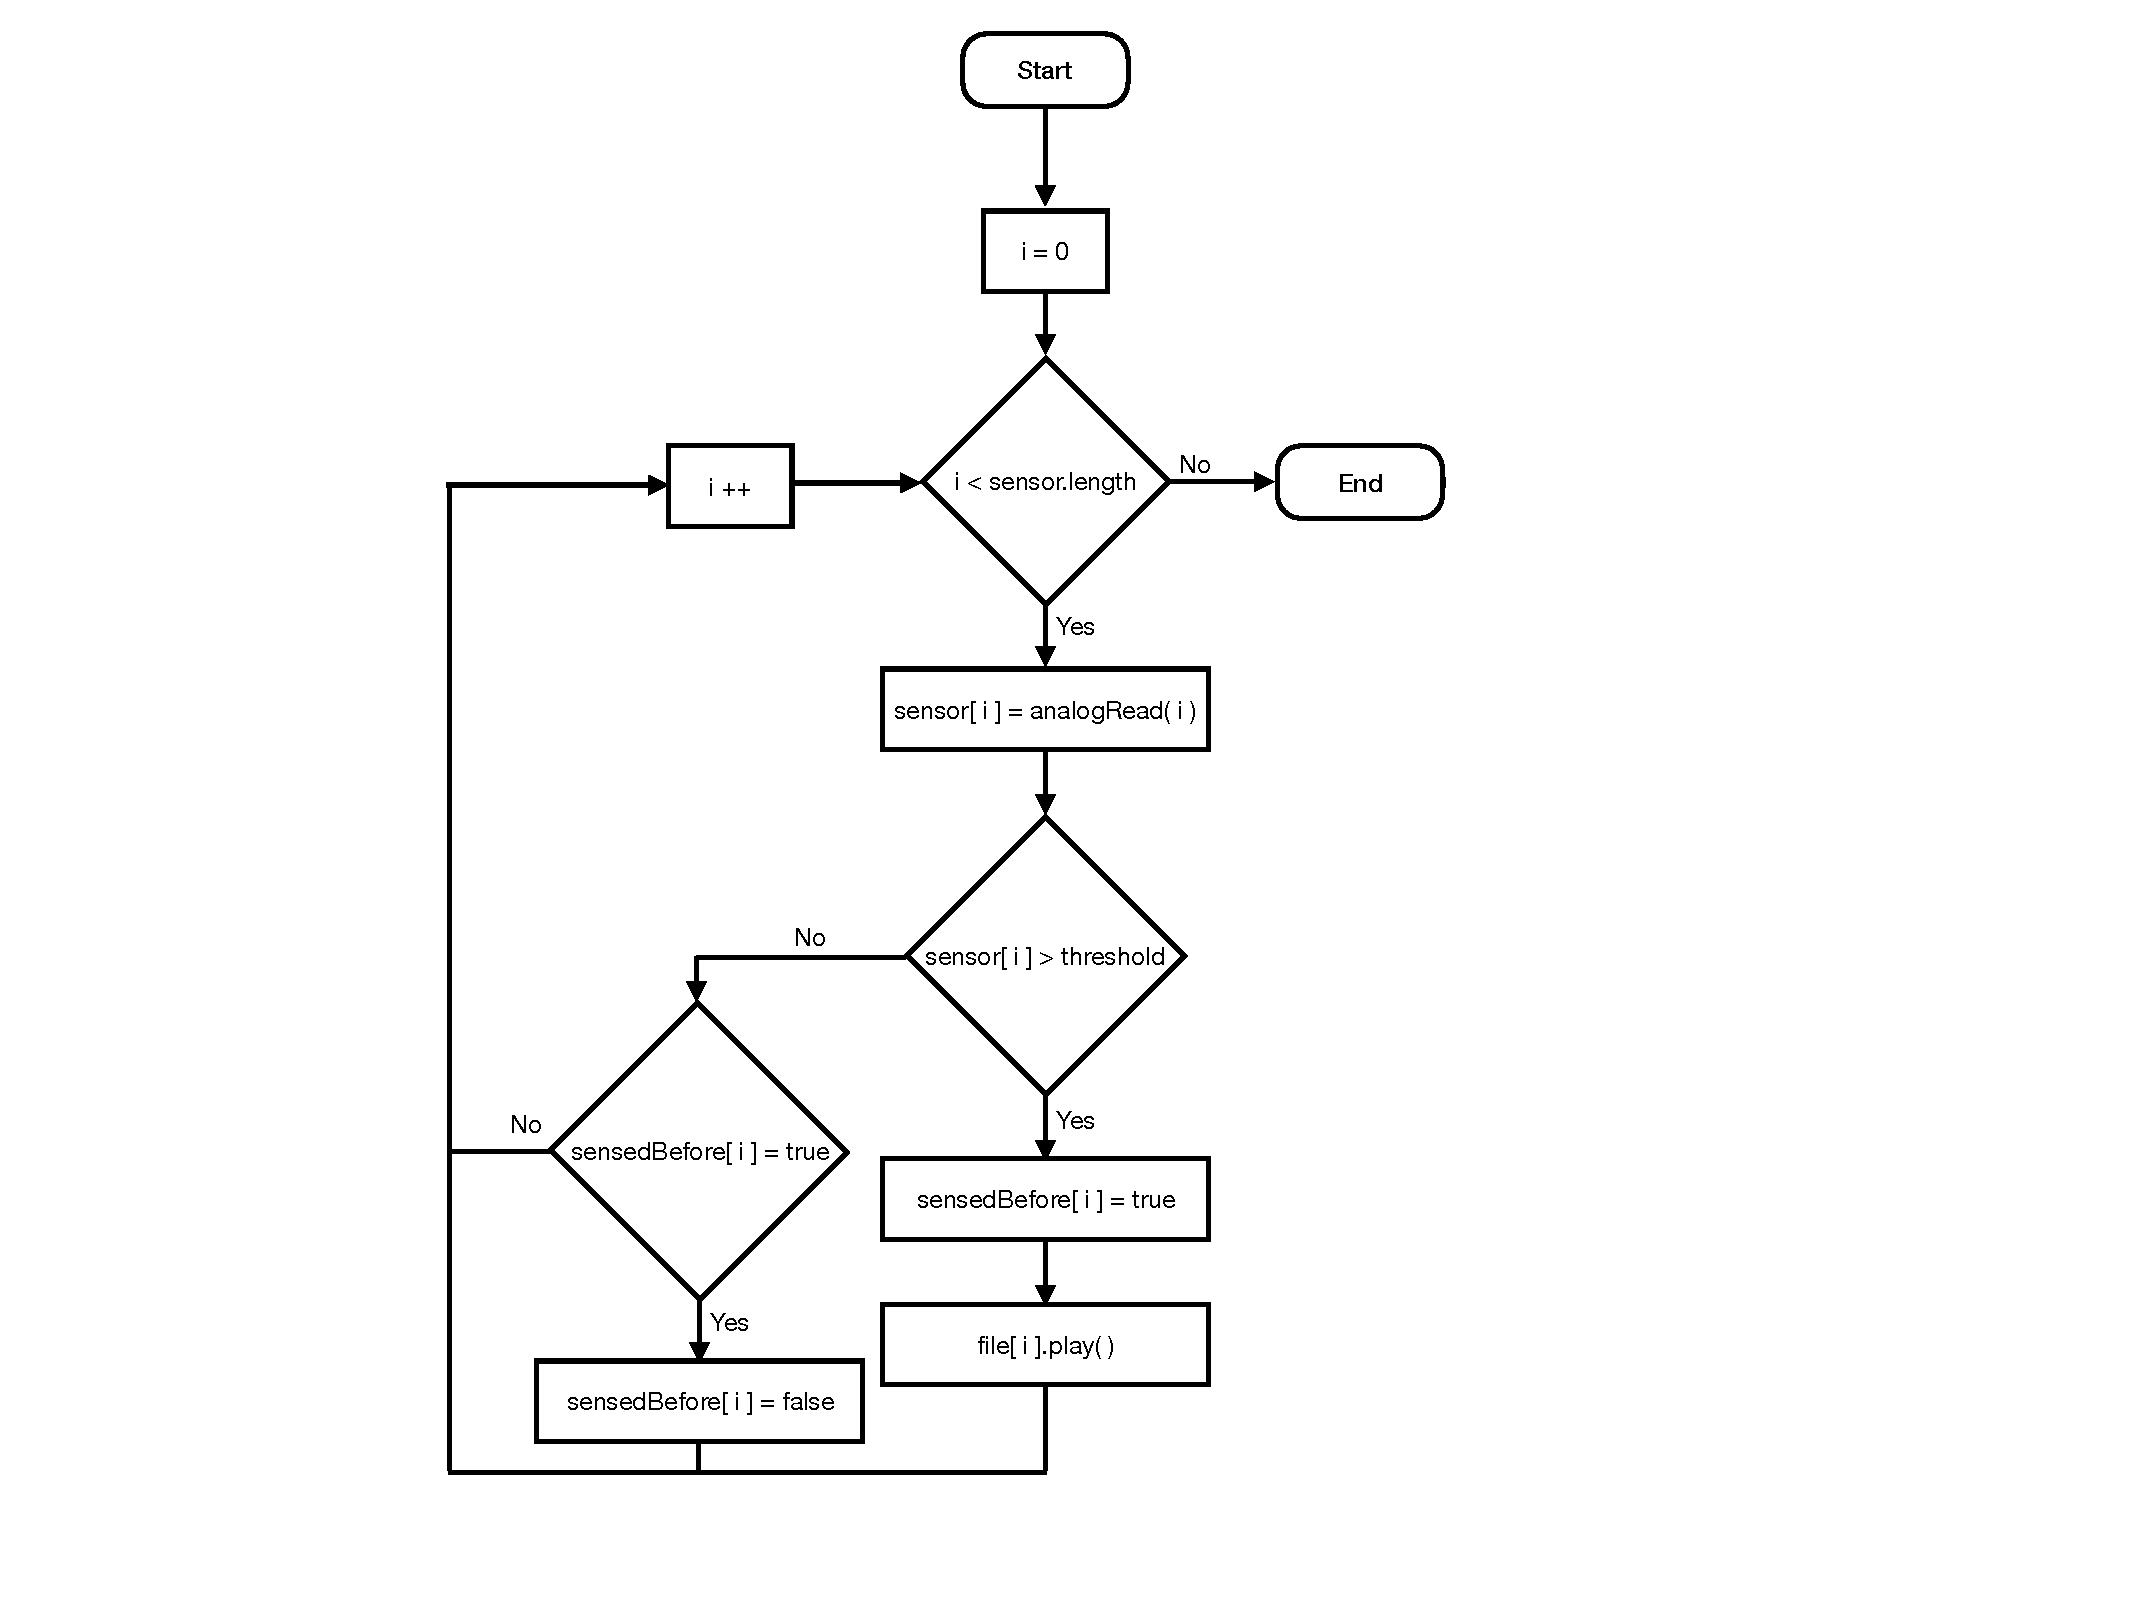
\includegraphics[scale=0.5]{Figure/protoFlowChart03.pdf}
\caption{
Flowchart for funktionen Afspil lyd. }
\label{fig:protoFlowChart03.pdf}
\end{figure}

 